\section{Experiment}
We applied this search strategy to dataset generated by the classic lamination
theory and failure theories. In this dataset, sixtheen attribues and two actual
values are given.
\subsection{Dataset Preparation}
Equation \ref{equ:stress-strain} takes an analytical approach to model the
relationship between stress and strain. We sample this function to yield 14000 points
uniformly distributed over the domain space.

The range of in-plane loading is from 0 to 120; the range of fiber orientation $\theta$ is from
-90 to 90; ply thickness $t$ is 1.27mm, number of plies range $N$ is from 4 to 120;
Three different material is used in this experiment, as shown in table \ref{tab:mat}.
Figure \ref{tab:traing-data} shows part of the training data.

In order to speeds up the learning and accerlate convergence, the input
atttributes of the data set are rescaled to between 0 and 1.0 by a linear function.

\begin{table*}[!t]	
\centering
\caption{Examples of the training data}
\label{tab:traing-data}
\begin{adjustbox}{width=1\textwidth}
	\begin{tabular}{cccc|cc}
		\toprule
		\multicolumn{4}{c}{\textbf{Input}} &  \multicolumn{2}{c}{\textbf{Output}} \\
		\midrule
		Load  &  \makecell{Laminate \\ Structure }  & \makecell{Material \\ Property} & \makecell{Failure \\  Property}  & MS & Tsai-Wu \\
		\midrule

		-70,-10,-40,  & 90,-90,4,1.27, & 38.6,8.27,0.26,4.14,  & 1062.0,610.0,31,118,72,  & 0.0102, & 0.0086 \\
		-10,10,0,     & -86,86,80,1.27,& 181.0,10.3,0.28,7.17, & 1500.0,1500.0,40,246,68, & 0.4026, & 2.5120 \\
		-70,-50,80,   & -38,38,4,1.27, & 116.6,7.67,0.27,4.173,& 2062.0,1701.0,70,240,105,& 0.0080, & 0.0325 \\
		-70,80,-40,   & 90,-90,48,1.27,& 38.6,8.27,0.26,4.14,  & 1062.0,610.0,31,118,72,  & 0.0218, & 0.1028 \\
		-20,-30,0,    & -86,86,60,1.27,& 181.0,10.3,0.28,7.17, & 1500.0,1500.0,40,246,68, & 0.6481, & 0.9512 \\
		0,-40,0,      & 74,-74,168,1.27,& 181.0,10.3,0.28,7.17,& 1500.0,1500.0,40,246,68, & 1.3110, & 3.9619 \\
		\bottomrule
		\end{tabular}
\end{adjustbox}
\end{table*}

\begin{table*}[!ht]
\caption{Properties of T300/5308 carbon/epoxy composite}
\label{tab:T300/5308}
\begin{adjustbox}{width=1\textwidth}
\centering
\begin{tabularx}{0.8\textwidth}{p{0.4\textwidth}p{0.1\textwidth}p{0.1\textwidth}c}
	\toprule
	\textbf{Property}								   & \textbf{Symbol}				  & \textbf{Unit}  & \textbf{ Graphite/Epoxy}     \\
	\midrule
	Longitudinal elastic modulus			   & $E_1$				  & GPa   &  181                 \\
	Traverse elastic modulus				   & $E_2$				  & GPa   &  10.3                \\
	Major Poisson's ratio					   & $v_{12}$			  &       &  0.28                \\
	Shear modulus							   & $G_{12}$			  & GPa   &  7.17                \\
	Ultimate longitudinal tensile strength     & $(\sigma_1^T)_{ult}$ & MP    &  1500                 \\
	Ultimate longitudinal compressive strength & $(\sigma_1^C)_{ult}$ & MP    &  1500                 \\
	Ultimate transverse tensile strength       & $(\sigma_2^T)_{ult}$ & MPa   &  40                   \\
	Ultimate transverse compressive strength   & $(\sigma_2^C)_{ult}$ & MPa   &  246                   \\
	Ultimate in-plane shear strength           & $(\tau_{12})_{ult}$  & MPa   &  68                    \\
	\bottomrule
\end{tabularx}
\end{adjustbox}
\end{table*}



\begin{figure}[h!]
	\centering
	\begin{subfigure}[b]{1.0\linewidth}
		\centering
		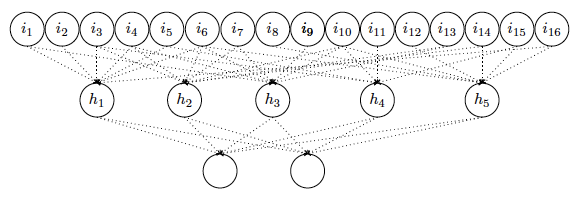
\includegraphics[width=0.8\textwidth]{fig/experiment_architecture_example1.png}
    	%%\begin{figure}
%\centering
\begin{tikzpicture}
	[ p/.style={ draw=none, fill=none}, 
	  remember picture, 
	  net/.style={ matrix of nodes, nodes={ draw, circle, inner sep=7.5pt },
	  nodes in empty cells,
	  column sep=-10.5pt,
	  row sep=0.8cm,
	  },
	  scale=0.6,
	  every node/.style={}
	]
%\draw[help lines] (-3cm,-6cm) grid (6cm,3cm);
\matrix[net] (mat)
{
		  & |[p]| &  & |[p]| &  & |[p]| &  & |[p]| &  & |[p]| &  & |[p]| &  & |[p]| &  & |[p]| &  &
			|[p]| &  & |[p]| &  & |[p]| &  & |[p]| &  & |[p]| &  & |[p]| &  & |[p]| &  & |[p]|    \\
	 |[p]| & |[p]| & |[p]| &  |[p]| &        & |[p]| & |[p]| & |[p]| &|[p]| &       & |[p]| &  |[p]| & |[p]| &
	 |[p]| &       & |[p]| &  |[p]| &  |[p]| & |[p]| & |[p]| &       &|[p]| & |[p]| & |[p]| & |[p]|
		   & |[p]| &       &  |[p]| &  |[p]| & |[p]| & |[p]| & |[p]| &|[p]| \\ 
	 |[p]| &  |[p]| & |[p]|  &  |[p]| & |[p]|  &  |[p]| &  |[p]| &  |[p]| & |[p]| & |[p]| & |[p]| &       & |[p]|
		   &  |[p]| & |[p]|  &  |[p]| &        &  |[p]| &  |[p]| &  |[p]| & |[p]| & |[p]| & |[p]| & |[p]| &     |[p]|
		   &  |[p]| & |[p]|  &  |[p]| & |[p]|  &  |[p]| &  |[p]| &  |[p]| \\ 
	  };
	  \node at (mat-1-1.base)  {$i_1$};
	  \node at (mat-1-3.base)  {$i_2$};
	  \node at (mat-1-5.base)  {$i_3$};
	  \node at (mat-1-7.base)  {$i_4$};
	  \node at (mat-1-9.base)  {$i_5$};
	  \node at (mat-1-11.base)  {$i_6$};
	  \node at (mat-1-13.base)  {$i_7$};
	  \node at (mat-1-15.base)  {$i_8$};
	  \node at (mat-1-17.base)  {$i_9$};
	  \node at (mat-1-17.base)  {$i_9$};
	  \node at (mat-1-19.base)  {$i_{10}$};
	  \node at (mat-1-21.base)  {$i_{11}$};
	  \node at (mat-1-23.base)  {$i_{12}$};
	  \node at (mat-1-25.base)  {$i_{13}$};
	  \node at (mat-1-27.base)  {$i_{14}$};
	  \node at (mat-1-29.base)  {$i_{15}$};
	  \node at (mat-1-31.base)  {$i_{16}$};

	  \node at (mat-2-5.base)  {$h_1$};
	  \node at (mat-2-10.base) {$h_2$};
	  \node at (mat-2-15.base) {$h_3$};
	  \node at (mat-2-21.base) {$h_4$};
	  \node at (mat-2-27.base) {$h_5$};
		 \foreach \a in {1,3,5,7,9,11,31}{
				\draw[->,dotted] (mat-1-\a.south) -- (mat-2-5.north);
			 }
		 \foreach \a in {5,7,11,13,19,25,27}{
				\draw[->,dotted] (mat-1-\a.south) -- (mat-2-10.north);
			 }
		 \foreach \a in {1,7,11,13,17,19,25}{
				\draw[->,dotted] (mat-1-\a.south) -- (mat-2-15.north);
			 }
		 \foreach \a in {5,9,19,21,29}{
				\draw[->,dotted] (mat-1-\a.south) -- (mat-2-21.north);
			 }
		 \foreach \a in {11,15,19,23,27,29,31}{
				\draw[->,dotted] (mat-1-\a.south) -- (mat-2-27.north);
			 }
		 \foreach \c in {5,10,15,21,27}{
			\foreach \d in {12,17}{
				\draw[->,dotted] (mat-2-\c.south) -- (mat-3-\d.north);
			}
 }
\end{tikzpicture}
%\caption{Parent 1\label{fig:parents1}}
%\end{figure}

		\caption{Parent 1}
		\label{fig:p1}
	\end{subfigure}
	\newline
	\begin{subfigure}[b]{1.0\linewidth}
		\centering
		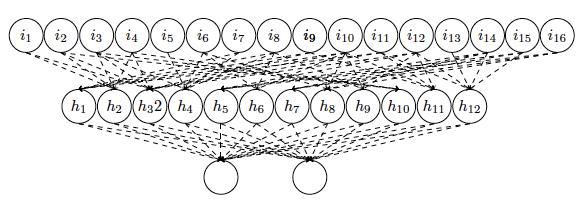
\includegraphics[width=0.8\textwidth]{fig/experiment_architecture_example2.png}
		\caption{Parent 2}
		\label{fig:p2}
	\end{subfigure}
	\newline
	\begin{subfigure}[b]{1.0\linewidth}
		\centering
		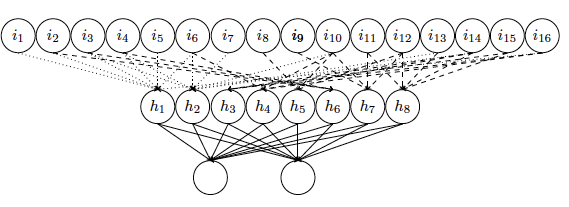
\includegraphics[width=0.8\textwidth]{fig/experiment_architecture_child.png}
		\caption{Child}
		\label{fig:child}
	\end{subfigure}
	\caption{Search Operation}
	\label{fig:search}
\end{figure}
